\label{cha:background-cscl}
In Chapter \ref{chapter:introducao}, we briefly introduced some aspects of Computer-Supported Collaborative Learning (CSCL). 
In this chapter will provide a better overview on CSCL background. 
Firstly, we will present some considerations about CSCL and related topics, as intentional design, CSCL scripts, and interaction patterns, for instance. 
Secondly, we will provide an overview of the efforts the CSCL community has been doing to improve group formation (GF). 
More specifically, We are concerned with how groups have been created, what criteria to cluster learners in groups have been most investigated, and what are the rationale behind the selection of such criteria. 
Finally, in the last section we will make some considerations.

There are several definitions and/or related concepts around collaborative learning (CL) in the literature. 
In this thesis, the term collaborative learning is used to refer to students working in intentionally designed groups. 
We are aware that there are situations where teachers ask students to form groups and work together freely, however, free collaboration does not necessarily leads to learning gains \cite{An_Ontological_Engineering_Approach_tese}, and several researchers have already reported that ill-designed CL activities can lead to unsuccessful group learning \cite{Motivation_in_a_computer-supported_collaborative_learning}. 
CL benefits can be enhanced when technological support is provided. 
So, CSCl is a pedagogical approach that can foster learning by providing to the learners situations to study in groups. 
In such approach, computers are tools that support the learning process and social interactions \cite{CSCL_historical_perspective}. 

Current research on CSCL have investigated how to scaffold learners interactions, 

Learning as a consequence of the planned 

So to be effective means, ...


% Learning in social process
\begin{figure}[h!]
\caption{“.}
\centering
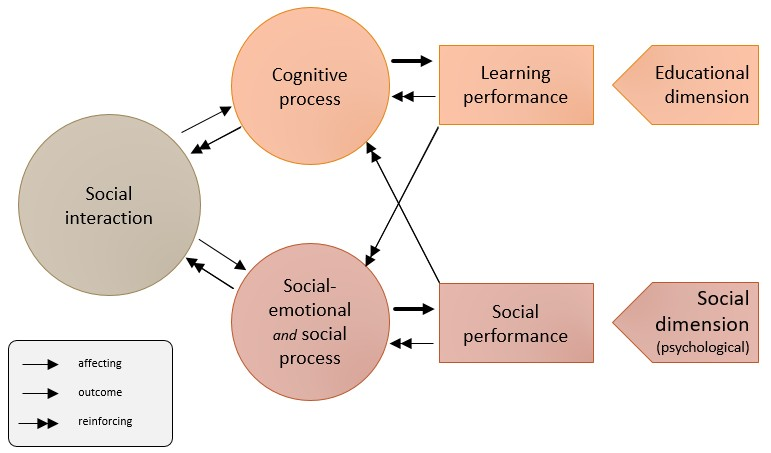
\includegraphics[width=0.7\textwidth]{social_interaction}
\label{fig:social_interaction}
\end{figure}

\section{CSCL Scripts}

\section{Interaction Patterns}

\subsection{Interaction Patterns based on Collaborative Learning Techniques}

\subsection{Interaction Patterns based on Learning Theories}

\section{Group Formation}
There are several denominations for the act of grouping learners in the context of collaborative learning, such as, group/team composition (Hsu et al. 2008) group or team formation (Yannibelli and Amandi 2012), grouping students (Alfonseca et al. 2006), clustering students (Chiu and Hsiao 2010).
Basically, these denominations have the same meaning, as the act of bringing together students in effective learning groups (Isotani et al. 2009). 
In this thesis, we adopt the term group formation, which is the most widely term used in the investigated studies.
Although the term "effective" can have different meanings among researchers, in this field is often used as a synonym for the proper allocation of resources to enhance the learning process (Isotani et al. 2009). 
These resources can be tangible (e.g. learning materials and tools to support collaboration) or intangible (e.g. knowledge and skills to be learned). 
Most research on group formation have focused on how to allocate these resources based on the learners profiles, on the technologies involved, or on the tasks to be performed (CL techniques, also knows as CL best practices) (Magnisalis et al. 2011).

Using learners' profiles helps instructors adequately deliver custom content to satisfy, not only individual necessities of the learners, but also group's necessities (Alfonseca et al. 2006; Faria et al. 2006; Greer et al. 1998; Ounnas et al. 2009; Graf and Bekele 2006), while inputs from the environment, can give more information that can help to understand the collaborative context and as a result, to improve grouping quality (Muehlenbrock 2005; Villasclaras-Fernández et al. 2009; Hernández-Leo et al. 2011; Wesner and Pfister 2001). 
Finally, there are other approaches for group formation that relies on using specifications of CL techniques to acquire sufficient information to group the learners (Isotani et al. 2009).

Generally, the formation of groups can be performed randomly (e.g. assigning learners in the groups by chance), self-selected (i.e. the learners choose with whom they want to study), or it can be carried out by an instructor or computing system, based on some criteria (Ikeda and Mizoguchi 1997; Alfonseca et al 2006; Graf and Bekele 2006; Hsu and Chou 2008; Ounnas et al. 2009; Boticki et al. 2013; Greer et al. 1998; Faria et al. 2006)
As discussed by (Dillenbourg and Jermann 2007) and (Laurillard 2009), the benefits of collaborative learning arise only when there is a detailed and proper planning of components and collaborative mechanisms. 
Considering these, many authors have raised concerns regard random selection and self-selected approaches since these approaches can result in unequal participation such as, students in the same group working at a different pace, off-task behavior, or even increasing students’ resistance to group work (Barkley et al. 2005; Dillenbourg 2002; Isotani and Mizoguchi 2008; ).
Moreover, one way to increase the chances of forming groups more capable to achieve the desired learning goals is assigning learners to groups using approaches based on CL techniques (Barkley et al. 2005; Dillenbourg 2002; Stahl 2004; Isotani et al. 2009).

%-------------------------------------------------------
% Concluding Remarks
%-------------------------------------------------------
\section{Concluding Remarks}

Regardless of the strategy used, the research in the area sought to investigate ways to influence positively the behavior of individuals to form groups where their presence and that of their peers are relevant; that interactions are significant; and to maximize the chances that knowledge construction will occur in more favorable conditions. 